%% Latex template for PhD dissertation or MS thesis
%% Department of Electrical and Computer Engineering
%% Brigham Young University
%% Last Modified: July 2017 by mdr@byu.edu

\documentclass[12pt,oneside]{report}
% generate the one-sided version: this is the ETD version
% print the one-sided version one sided for all the department and college approvals

% \documentclass[12pt,twoside]{report}
% Uncomment this line (and comment line 6) to create the two-sided version.
% Print the two-sided version two-sided for the optional printed and bound version.

%%%%%%%%%%%%%%%%%%%%%%%%%%%%%%%%%%%%%%%%%%%%%%%%%%%%%%%%%
%  Setup BYU thesis format
%%%%%%%%%%%%%%%%%%%%%%%%%%%%%%%%%%%%%%%%%%%%%%%%%%%%%%%%%
\usepackage{byustyle}
% Setup the byu style sheet
\byustylesetup{%
    %
    isdissertation = true,            % false for MS thesis, true for PhD dissertation
	%
    % Definitions of names needed in thesis/dissertation
    deptname          = Department of Civil ann Environmental Engineering,
    committeechairman = Michael A. Scott,
    committeemembera  = Michael J. Borden,
    committeememberb  = Brian A. Mazzeo,
	committeememberc  = Brad L. Hutchings, % needed for dissertation, ignored for thesis
	committeememberd  = Steven M. Schultz,    % needed for dissertation, ignored for thesis
    %
    %Change true/false to shorten for proofreading purposes
    noabstract = false,         % Do not show the abstract page
    nouniversitypages = false,  % Do not show any of the "university pages"
    noacknowledgements = false, % Do not show the Acknowledgements page
    notableofcontents = false,  % Do not show the Table of Contents
    nolistoffigures = false,    % Do not show the List of Figures
   	nolistoftables = false,     % Do not show the List of Tables
    nonomenclature = true,      % Do not show the Nomenclature section - note that this section is optional
    notocandlists = false,      % Do not show the Table of Contents, List of Figures, or the List of Tables
    noheaderatall = false,      % Do not show any of the BYU Thesis header pages
    keywords = {thesis template, dissertation template, technical writing} % your keywords
}

%%%%%%%%%%%%%%%%%%%%%%%%%%%%%%%%%%%%%%%%%%%%%%%%%%%%%%%%
% Package inclusions go here
% The list starts with some commonly used packages
% That do not conflict with byutyle.sty
%%%%%%%%%%%%%%%%%%%%%%%%%%%%%%%%%%%%%%%%%%%%%%%%%%%%%%%%

\usepackage{amsmath}					%	allows for mathematical symbols
\usepackage{amssymb}					%	defines symbol names for all the math symbols
\usepackage{graphicx}        			% for .pdf graphics inclusion
\usepackage[calcwidth = \columnwidth]{caption}
\usepackage{booktabs,threeparttable}
\usepackage{setspace}					%	change the spacing inside a document
\usepackage{epstopdf}					%	converts a .eps to a .pdf
\usepackage{cite}						%	allows for citations
\usepackage{float}						%	improves the interface for defining floating objects
\usepackage{rotating}
\usepackage{printlen}

%%%%%%%%%%%%%%%%%%%%%%%%%%%%%%%%%%%%%%%%%%%%%%%%%%%%%%%%%%%%%%%%%%%%
%  Include additional \usepackage{} statements here.
%    Add one package at a time.
%    Warning:  Some packages are not compatible with byustyle.sty
%%%%%%%%%%%%%%%%%%%%%%%%%%%%%%%%%%%%%%%%%%%%%%%%%%%%%%%%%%%%%%%%%%%

%These next two lines are for the citing with the IEEE style
\renewcommand\citepunct{], [}
\renewcommand\citedash{]--[}

%%%%%%%%%%%%%%%%%%%%%%%%%%%%%%%%%%%%%%%%%%%%%%%%%%%%%%%%
% For doing bookmarks in the PDF file
%%%%%%%%%%%%%%%%%%%%%%%%%%%%%%%%%%%%%%%%%%%%%%%%%%%%%%%%%
% For more info, see:
% http://www.geocities.com/kijoo2000/latex2pdf.pdf
% http://www.tug.org/applications/hyperref/manual.html
\usepackage[pdftex,backref,pagebackref,plainpages=false]{hyperref}
\hypersetup{
    %bookmarks    = true, % Make bookmarks (default=true). This option
                          %cannot be used after package has been loaded,
                          %thus use like this: \usepackage[bookmarks=false]{hyperref}.
    %
    breaklinks   = false, % Allow link text to break across lines (default=false).
    linktocpage  = false, % make page number, not text, be link on TOC, LOF and LOT
    colorlinks   = false, % Color the text of links (true) or put color frames over
    %
    linkbordercolor  = {1 1 1}, % The color of the box around normal links (white so they won't show up)
    citebordercolor  = {1 1 1}, % The color of the box around citations (white so they won't show up)
                          % the links (false).
    pdfstartview = {FitV}, % Set the startup page view. Possible options are:
                           % FitH: Fit whole width of page
                           % FitV: Fit whole height of page
                           % FitB: Fit whole �Bounding Box� page
                           % FitBH: Fit whole width of �Bounding Box� of page
                           % FitBV: Fit whole height of �Bounding Box� of page
    bookmarksnumbered  = true, % Put section numbers in bookmarks (default=false)
    bookmarksopen      = true, % Open up the bookmark trees (default=false).
    bookmarksopenlevel = 0, % Level to which bookmarks are open (default=\maxdimen).
    bookmarkstype      = toc, % Specify which toc file to mimic (default=toc).
    pdfpagemode        = {UseOutlines}, %  Specify how document starts when opened ({None}).
                                        % Possible options are:,
                                        % None: Neither bookmarks nor thumbnails are visible.
                                        % UseOutlines: Bookmarks are visible.
                                        % UseThumbs: Thumbnails are visible.
                                        % FullScreen: Full-screen mode
    pdftitle    = {Thesis},
    pdftitle    = {First Line of your Thesis/Dissertation Title},
    pdfauthor   = {Isaac Newton},
    pdfcreator  = {Isaac Newton},
    pdfsubject  = {Isaac Newton's Master's Thesis},
    pdfkeywords = {Master's Thesis, BYU},
    pdfborder		=	{0 0 0},}

%%%%%%%%%%%%%%%%%%%%%%%%%%%%%%%%%%%%%%%%%%%%%%%%%%%%%%%%
%  Define macros here - You may use these, or delete them, as you see fit.
%%%%%%%%%%%%%%%%%%%%%%%%%%%%%%%%%%%%%%%%%%%%%%%%%%%%%%%%%

% \def\proof{\noindent{\it Proof: }}
% \def\QED{\mbox{\rule[0pt]{1.5ex}{1.5ex}}}
% \def\endproof{\hspace*{\fill}~\QED\par\endtrivlist\unskip}
% \newcommand{\norm}[1]{\left\|#1\right\|}
\newcommand{\abs}[1]{\left|#1\right|}
% \newcommand{\defeq}{\stackrel{\triangle}{=}}
% \newcommand{\re}{\mathbb{R}} 		% real numbers
% \newcommand{\OMIT}[1]{{}} 		% omit sections of text
\newcommand{\pd}[2]{\ensuremath{\frac{\partial #1}{\partial #2}}} % partial derivative
% \newcommand{\superscript}[1]{\ensuremath{^\textrm{#1}}}
% \newcommand{\subscript}[1]{\ensuremath{_\textrm{#1}}}


%%%%%%%%%%%%%%%%%%%%%%%%%%%%%%%%%%%%%%%%%%%%%%%%%%%%%%
% Define the 'inverted pyramid' table caption
% requirement from the College.
%%%%%%%%%%%%%%%%%%%%%%%%%%%%%%%%%%%%%%%%%%%%%%%%%%%%%%

\DeclareCaptionJustification{InvertedPyramid}{\hsize=\linewidth
                \parindent=0pt
                \leftskip=0pt plus.5fil
                \rightskip=0pt plus-0.5fil
                \parfillskip=0pt plus1fil
                \emergencystretch=1in
                \parshape10
                0.00in \linewidth
                0.025\linewidth 0.95\linewidth
                0.05\linewidth 0.9\linewidth
                0.075\linewidth 0.85\linewidth
                0.1\linewidth 0.8\linewidth
                0.125\linewidth 0.75\linewidth
	     0.15\linewidth 0.70\linewidth
	     0.175\linewidth 0.65\linewidth
	     0.2\linewidth 0.60\linewidth
	     0.225\linewidth 0.55\linewidth
                \strut
	} 
\renewcommand{\TPTminimum}{3in}
\captionsetup[table]{justification=InvertedPyramid} 

\newsavebox{\tempbox}
\newlength{\tempwidth}

%%%%%%%%%%%%%%%%%%%%%%%%%%%%%%%%%%%%%%%%%%%%%%%%%%%%%%%%%%%%%%%%%%%%
% To only print a few chapters without changing the reference numbers
% (Consult your favorite LaTeX resource.) 
%%%%%%%%%%%%%%%%%%%%%%%%%%%%%%%%%%%%%%%%%%%%%%%%%%%%%%%%%%%%%%%%%%%%
%\includeonly{...}

%%%%%%%%%%%%%%%%%%%%%%%%%%%%%%%%%%%%%%%%%%%%%%%%%%%%%%%%
% Start Document
%%%%%%%%%%%%%%%%%%%%%%%%%%%%%%%%%%%%%%%%%%%%%%%%%%%%%%%%
\begin{document}

% Define Title
% For a title of more than one line, use the \\ to break up the lines so they appear in an inverse pyramid shape.
% Also, make sure you use title case 
\title{On Writing an MS Thesis\\Second Line of Title if Necessary\\Three Line Limit}

% Define author
\author{Di Miao}

% For displaying the BYU Thesis header
% 	This command assumes that there are documents called abstract.tex and
% 	acknowledgements.tex (and optionally nomenclature.tex) that will be 
%   included in the header
\showBYUHeader

% Include chapters of the thesis here: 
% The inludes are populated by example chapters
\chapter{Introduction}
\label{chp:chapter1}
\graphicspath{{figures/}{figures/chapter1/}}
\pgfplotsset{
    table/search path={{figures/chapter1/data},{data}},
}

In classical finite element analysis, $80\%$ of overall analysis time is devoted to mesh generation and cleanup, whereas only $20\%$ of overall time is actually devoted to analysis~\cite{cottrell2009isogeometric}. Isogeometric analysis, introduced by Hughes et al.~\cite{HUGHES20054135}, leverages computer aided design (CAD) representations directly in finite element analysis (see Figure~\ref{fig:flow_chart}). It has been shown that this approach can alleviate the model preparation burden of going from a CAD design to an analysis model and improve overall solution accuracy and robustness~\cite{bazilevs2006isogeometric, da2011some, da2014mathematical}. Additionally, the higher-order smoothness inherent in CAD basis functions make it possible to solve higher-order partial differential equations, e.g. the biharmonic equation~\cite{kapl_isogeometric_2015, kapl_isogeometric_2017}, the Kirchhoff-Love shell problem~\cite{kiendl2009isogeometric, kiendl2010bending, kiendl2015isogeometric} and the Cahn-Hilliard equation~\cite{gomez2008isogeometric, borden2014higher} directly without resorting to complex mixed discretization schemes.\par

\begin{figure}[ht]
	\captionsetup[subfigure]{labelformat=empty, font = footnotesize}
	\centering
	\begin{subfigure}[b]{0.47\textwidth}
		\centering
		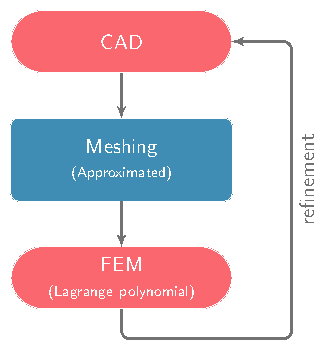
\includegraphics[scale=1.2]{flow-chart-fem}
		\caption{FEA workflow}
	\end{subfigure}
	\begin{subfigure}[b]{0.47\textwidth}
		\centering
		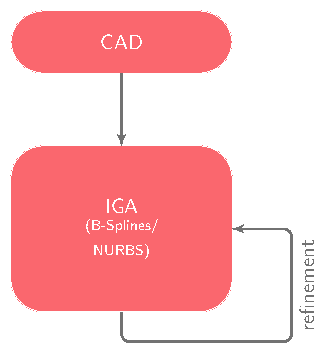
\includegraphics[scale=1.2]{flow-chart-iga}
		\caption{IGA workflow}
	\end{subfigure}
	\caption{A comparison of between classical finite element analysis workflow and isogeometric analysis workflow. FEA workflow: meshing and cleanup are required. Note that the meshing process does not preserve the original CAD geometry. IGA workflow: using the CAD model directly in the finite element analysis. }
	\label{fig:flow_chart}
\end{figure}

CAD models are often built from collections of non-uniform rational B-splines (NURBS). Adjacent NURBS patches often have inconsistent knot layouts, different parameterizations, and may not even be physically connected. Additionally, trimming curves~\cite{kim2009isogeometric, schmidt2012isogeometric} are often employed to further simplify the design process and to extend the range of objects that can be modeled by NURBS at the expense of further complicating the underlying parameterization of the object. While usually not an issue from a design perspective, these inconsistencies in the NURBS patch layout, including trimming, must be accommodated in the isogeometric model to achieve accurate simulation results. As shown in Figure~\ref{fig:geometries}, two primary approaches are often employed. First, the exact trimmed CAD model, shown in Figure~\ref{fig:geometries} in the middle, is used directly in the simulation~\cite{schmidt2012isogeometric}. To accomplish this requires additional algorithms for handling cut cells and the weak imposition of boundary conditions and may result in reduced solution accuracy and robustness. Second, the CAD model is reparameterized~\cite{xu2014high}, as shown in Figure~\ref{fig:geometries} on the right, into a watertight spline representation like multi-patch NURBS, subdivision surfaces~\cite{peters2008subdivision}, or T-splines~\cite{sederberg_t-splines_2003} which can then be used as a basis for analysis directly. The reparameterization process often results in more accurate and robust simulation results but is only semi-automatic using prevailing approaches. In both cases, existing techniques are primarily surface-based due to the predominance of surface-based CAD descriptions.

\begin{figure}[ht]
	\captionsetup[subfigure]{labelformat=empty, font = footnotesize}
	\centering
	\begin{subfigure}[b]{0.32\textwidth}
		\centering
		\includestandalone[scale=.7]{geometry}
		\caption{A geometry}
	\end{subfigure}
	\begin{subfigure}[b]{0.32\textwidth}
		\centering
		\includestandalone[scale=.7]{trimmed_geometry}
		\caption{Trimmed model}
	\end{subfigure}
	\begin{subfigure}[b]{0.32\textwidth}
		\centering
		\includestandalone[scale=.7]{reparameterized_geometry}
		\caption{Reparameterized model}
	\end{subfigure}
	\caption{A geometry and two modelling strategies: trimming and reparameterization.}
	\label{fig:geometries}
\end{figure}

From the analysis perspective, the main challenge for conducting finite element analysis over a geometry consisting of multiple spline patches is how to efficiently and accurately exchange information among different patches. In this dissertation, we focus on the \textit{dual mortar method}, which can robustly apply constraints over intersections of reparameterized multi-patch geometries.  

\section{State of the art}

Researchers in both the design and analysis communities have made significant progress in handling multi-patch NURBS models and the connections between adjacent patches. In this section, we present a brief review of patch coupling techniques developed in both communities. 
\subsection{Local refinable splines}

\begin{figure}[h]
    \centering
    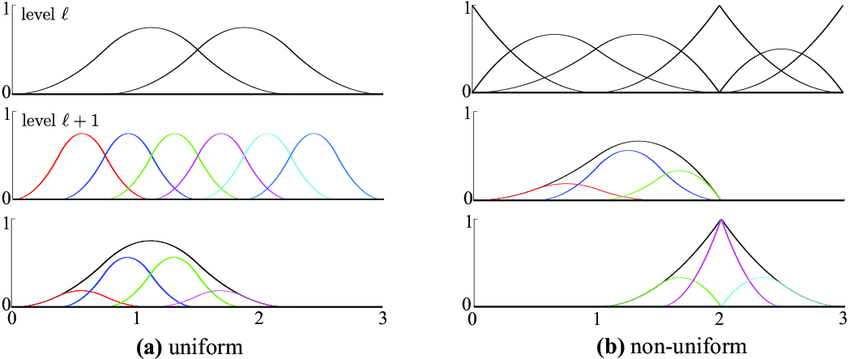
\includegraphics[width=.8\linewidth]{hierarchical-bsplines}
    \caption{Subdivision of B-spline basis functions: (a) Uniform, and (b) non-uniform B-spline basis functions are represented by linear combinations of refined basis functions~\cite{hennig2016bezier}.}\label{fig:hierarchical-bsplines}
\end{figure}

 In order to represent complex topologies, subdivision schemes (Figure.~\ref{fig:hierarchical-bsplines}) are widespread in geometry processing and computer graphics. Subdivision schemes allow for the construction of smooth spline bases over unstructured meshes. Among the most popular subdivision schems are the Catmull-Clark \cite{catmull_recursively_1978}, Doo-Sabin \cite{doo_behaviour_1978} and Loop's \cite{loop_smooth_1987} scheme. For isogeometric analysis, Wei \textit{et al.} \cite{wei_truncated_2015} introduced truncated hierarchical Catmull-Clark subdivion that can handle extraordinary nodes involved in complex topologies. Truncated hierarchical Catmull-Clark subdivion inherits the surface continuity of Catmull-Clark subdivision, namely $C^1$ continuity at extraordinary points and $C^2$ continuity elsewhere. Loop subdivision surfaces provide similar regularity properties as truncated hierarchical Catmull-Clark subdivion and have been applied to isogeometric analysis in \cite{kang_truncated_2016,pan_isogeometric_2015} to generate triangular meshes. One of the limitations in the implementation of subdivision meshes is that the basis function around the extraordinary point is composed of piecewise polynomial functions with an infinite number of segments, which leads to insufficient integration by Gauss quadrature. To deal with this issue, various quadrature rules and adaptive strategies have been examined in \cite{nguyen_comparative_2014} for the Poisson problem on the disk and in \cite{juttler_numerical_2016} for fourth order partial differential equations. \par

\begin{figure}[h]
    \centering
    \begin{subfigure}[b]{0.45\textwidth}
        \centering
        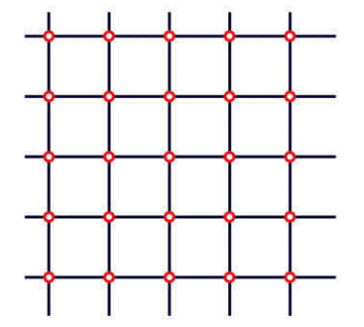
\includegraphics[width=\linewidth]{bspline-control-grid}
        \caption{B-splines}
    \end{subfigure}
    ~
    \begin{subfigure}[b]{0.45\textwidth}
        \centering
        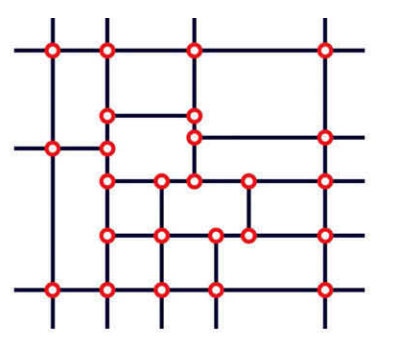
\includegraphics[width=\linewidth]{tspline-control-grid}
        \caption{T-splines}
    \end{subfigure}   
    \caption{Control points lie in a rectangular grid. (a) Topology of B-spline control grid. (b) Topology of T-spline
    control grid, the presence of T-junction control points is allowed~\cite{bazilevs_isogeometric_2010}.}\label{fig:Tspline-control-grid}
\end{figure}

\begin{figure}[h]
    \centering
    \begin{subfigure}[b]{0.45\textwidth}
        \centering
        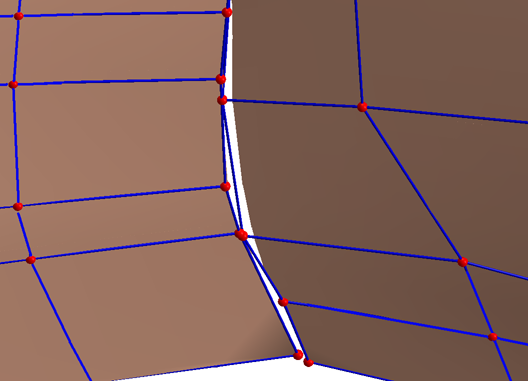
\includegraphics[width=\linewidth]{bspline-two-patch}
        \caption{B-splines}
    \end{subfigure}
    ~
    \begin{subfigure}[b]{0.45\textwidth}
        \centering
        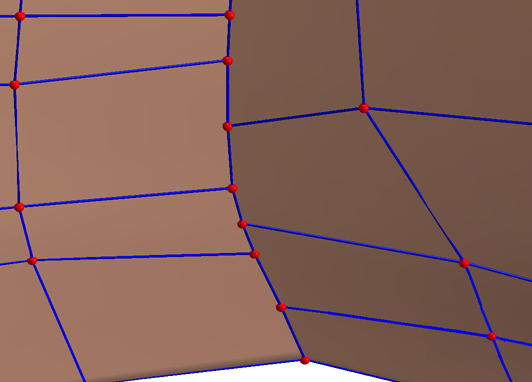
\includegraphics[width=\linewidth]{tspline-two-patch}
        \caption{T-splines}
    \end{subfigure}   
    \caption{A gap between two B-spline surfaces, fixed with a T-spline~\cite{sederberg_t-splines_2003}.}\label{fig:Tspline-two-patch}
\end{figure}

In 2003, Sederberg \textit{et al.} \cite{sederberg_t-splines_2003} introduced T-splines, which allow for the existence of T-junctions in the mesh, so that lines of control points need not traverse the entire mesh. Thus, local refinement can be realized by introducing T-junctions (see Figure.~\ref{fig:Tspline-control-grid}) around interested region. Since the concept of T-splines is a generalization of NURBS technology, it can also be used to merge NURBS surfaces that have different discretizaitons at the intersection (see Figure.~\ref{fig:Tspline-two-patch}). Due to the desirable features of T-splines, Bazilevs \textit{et al.} \cite{bazilevs_isogeometric_2010} explored this technology in isogeometric analysis, and numerical results demonstrated its potential for solving structural and fluid problems. By utilizing the B\'ezier extraction operator, a finite element data structure for T-splines \cite{scott_isogeometric_2011} were developed to ease the incorporation of T-splines into existing finite element codes. However, it has been proven \cite{buffa_linear_2010} that the original definition of T-splines is not sufficient to ensure the linear independence of the basis functions. To circumvent this issue, analysis suitable T-splines \cite{li_linear_2012} were developed by applying an additional constraint that no two orthogonal T-junction extensions are allowed to intersect. Subsequently, the mathematical properties of analysis suitable T-splines were studied in \cite{li_analysis-suitable_2013,xin_li_properties_2015}, and it has been sucessfully applied to the boundary element method \cite{scott2013isogeometric}. Meanwhile, an adaptive local h-refinement algorithm with T-splines and a local refinement of analysis-suitable T-splines were introduced by D\"{o}fel \textit{et al.} \cite{dorfel_adaptive_2010} and Scott \textit{et al.} \cite{scott_local_2012}, respectively. However, for both algorithm, the refined mesh is not as local as one would hope and this problem might be severe in 3D.\par

\subsection{Multi-patch geometrically continuous functions}

One of the advantages of isogeometric analysis is that it provides basis functions with high smoothness, \textit{i.e.} for $p$-th order splines, they enjoy up to $C^{p-1}$ continuity within a single patch. Thus, it is possible to directly discretize differential operators of order higher than 2. However, continuity higher than $C^0$ for multi-patch discretization imposes significant difficulties. The conception of geometric continuity is a well-known and highly useful concept in geometric design \cite{peters_chapter_2002, peters_joining_1992}. The parametric continuity requires both the smoothness of the geometry and its parameterization, whileas the geometric continuity only requires the smoothness of the geometry. Hence, the geometric continuity of order $s$ ($G^s$ continuity) is a weaker continuity constraint as compared to $C^s$ parametric continuity. Bercovier \textit{et al.} \cite{bercovier_smooth_2014} has shown that for multi B\'ezier patches over an unstructured quadrilateral mesh, as long as the order of polynomial is high enough, there always exists the minimal determining set for a $G^1$ continuity construction. Moreover, the resulting basis functions do not contain subdivisions around extraordinary vetices.\par

The case of $G^1$ continuous functions on bilinearly parametrized two-patch B-spline domains was considered by Kapl \textit{et al.} \cite{kapl_isogeometric_2015}, where the $C^1$ basis functions are constructed and analyzed by numerical tests. It is shown that the space dimensionality heavily depends on the parameterization of two bilinear patch, and optimal convergence is observed on the biharmonic problem. However, over-constrained $C^1$ isogeometric spaces that cause sub-optimal convergence are also observed for certain configurations (\textit{e.g.} two-patch non-bilinear parameterizations and $C^{p-1}$ continuity within the patches for $p$-th order spline space). A theoretical analysis of the cause of this so-called $C^1$ locking phenomenon is provided in \cite{collin_analysis-suitable_2016}, where the analysis-suitable $G^1$ geometry parameterization that allows for optimal approximation of $C^1$ isogeometric spaces, is identified and verified by numerical examples. Kapl \textit{et al.} extended the construction of $G^1$ continuous functions to bilinearly parameterized multi-patch domains in \cite{kapl_isogeometric_2017}, where the simple explicit formulas for spline coefficients of $C^1$ basis function are derived and nested $C^1$ isogeometric spaces are generated. Recently, Kapl \textit{et al.} \cite{kapl_space_2017,kapl_space_nodate} explored the construction of $C^2$ isogeometric functions on multi-patch geometries and utilized the $C^2$ isogeometric spaces for $6$-th order PDE.\par

Although the geometrically continuous functions circumvent the use of subdivisions for domains with extraordinary vertices, the requirement of $C^0$ parameterization averts local mesh refinement, and lower continuity is required to avoid $C^1$ locking effect. Thus, its implementation can be complex and it may not be a potential candidate for analysis in more general situations.\par

\subsection{Variational approaches}

From the analysis perspective, the pointwise satisfaction of continuity constraints between adjacent patches is often unnecessarily rigorous. A reasonable approximation can be achieved even if these constraints are applied in a variational setting. The Lagrange multiplier method is a general framework which can be used to apply constraints to variational problems. In the context of isogeometric analysis, various types of Lagrange multiplier approaches have been applied to problems in solids~\cite{hesch_isogeometric_2012, seitz2016isogeometric} and fluids~\cite{bazilevs2012isogeometric}. While general in applicability, the solvability and optimality of the Lagrange multiplier method is significantly influenced by the \textit{inf-sup} condition~\cite{babuvska1973finite,boffi_mixed_2013}. In the context of domain coupling, to satisfy the \textit{inf-sup} condition, special modifications are needed when building the Lagrange multiplier space to ensure stability (see Figure~\ref{fig:mortar_basis}). This has been further studied in~\cite{bernardi_basics_2005, bernardi_domain_1993, belgacem_mortar_1998, barbosa1991finite} for finite element analysis and in~\cite{brivadis_isogeometric_2015} for isogeometric analysis. \par

Whereas the Lagrange multiplier method applies continuity constraint by Lagrange multipier, leading to a saddle point problem, the mortar method, first introduced by Bernardi~\cite{bernardi_domain_1993}, considers a constrained solution space and gives rise to a positive definite variational problem. Wohlmuth~\cite{wohlmuth2000mortar} used dual basis functions to discretize the Lagrange multiplier spaces, which further simplifies the mortar formulation. Dual basis functions for the piecewise linear elements are illustrated in Figure~\ref{fig:mortar_basis}. A dual mortar method for isogeometric analysis was first developed by Seitz et al.~\cite{seitz_isogeometric_2016}. \par

Applying constraints by the Lagrange multiplier method leads to a saddle point problem, of which the discrete Lagrange multiplier basis functions cannot be chosen independently of that of the primal variable and special treatment is required to ensure the solvability and optimality of the discretized system. The stiffness matrix for the discrete problem arising from the Lagrangian multiplier method always contains both positive and negative eigenvalues, for which iterative methods are known to be less efficient than for symmetric positive definite systems. The perturbed Lagrangian method alleviates these issues by appending a weighted quadratic penalty term to the energy functional. The main drawback of the perturbed Lagrangian method is the inconsistency with the original problem. It has been utilized in \cite{simo1985perturbed} for contact problems and \cite{dornisch2011boundary, apostolatos2015domain} for domain decomposition problems in the isogeometric analysis framework.\par

To fully circumvent the inf-sup condition for imposing Dirichlet boundary conditions by Lagrange multiplier, Barbosa et. al. \cite{barbosa1991finite} added a new penalty like term to the energy functional to enhance the stability. Unlike perturbed Lagrangian methods where the penalty term is inconsistent with the original problem, the new term proposed by Barbosa maintains the consistency. It has been demonstrated that there is a close connection with the stablized Lagrange multiplier method and Nitsche's method in the context of setting the Dirichlet boundary conditions \cite{stenberg1995some} and in the context of domain decomposition \cite{hansbo2005lagrange, hansbo_nitsches_2005, juntunen2015connection}. Tur et. al. \cite{tur2015modified} utilized this method to solve both small and large deformation contact problems and obtained optimal convergence rates for linear elements. To our knowledge, this method has not been applied in the isogeometric analysis framework yet. \par

The discontinuous Galerkin method (or Nitsche's method) was introduced in 1971 \cite{nitsche_uber_1971} for handling Dirichlet boundary conditions in the weak sense. The discontinuous Galerkin method resembles a mesh-dependent penalty method. Unlike the standard penalty method, which is not consistent unless the penalty coefficient goes to infinity, the discontinuous Galerkin method is consistent with the original problem. Moreover, no additional unknown (Lagrange multiplier) is needed and no discrete inf-sup condition must be fulfilled, contrarily to mixed methods. Meanwhile, additional terms are added into the weak form to ensure the ellipticity of the problem. The discontinuous Galerkin method has been widely studied in various aspects, including imposing boundary conditions \cite{hansbo_nitsches_2005}, domain decomposition \cite{becker_finite_2003} and contact problems \cite{chouly_symmetric_2015}. In the field of the isogeometric analysis, the discontinuous Galerkin method has been utilized to impose Dirichlet boundary conditions for trimmed spline meshes \cite{embar_imposing_2010}. The first article discussing the discontinuous Galerkin method based domain decomposition strategy was written by Apostolatos \textit{et al.} \cite{apostolatos_nitsche-type_2014}. Nguyen \textit{et al.} extended it to three-dimensional problems in \cite{nguyen_nitsches_2014}. Guo \textit{et al.} \cite{guo_nitsches_2015} proposed a Nitsche's method for coupling Kirchhoff-Love NURBS shell patches.\par

\begin{figure}
  \centering
  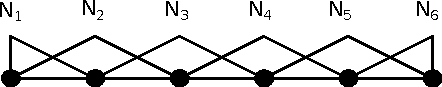
\includegraphics[width=.7\linewidth]{original_basis}\\
  \vspace{1em}
  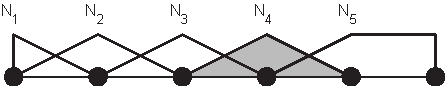
\includegraphics[width=.7\linewidth]{mortar_basis}\\
  \vspace{1em}
  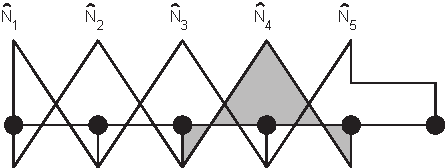
\includegraphics[width=.7\linewidth]{dual_mortar_basis}
  \caption{Lagrange multiplier basis functions for the piecewise linear elements, top: original piecewise linear basis, middle: piecewise linear basis with modification at the right end, bottom: dual basis functions for the piecewise linear elements, modification at the right end (Courtesy of Zienkiewicz~\cite{zienkiewicz1977finite}).}\label{fig:mortar_basis}
\end{figure}

\section{Research contributions}

In this dissertation, the dual mortar framework for most prevailing higher-order partial differential equations (including biharmonic problems, Cahn-Hilliard problems and Kirchhoff-Love shell problems) are developed. The primary contributions of this dissertation are:
\begin{itemize}
    \item Formulation and implementation of an isogeometric B\'ezier dual mortar method for the biharmonic problem on multi-patch domains. The formulation leads to an efficient construction of a sparse constrained linear system. We prove the well-posedness of the formulation and specify requirements to achieve optimal convergence. 
    \item Development of the enriched \Bezier dual basis. The enriched \Bezier dual basis functions are constructed via a quadrature-free algorithm and can reproduce polynomials up to a given degree. 
    \item Formulation and implementation of an isogeometric \Bezier dual mortar method for the Kirchhoff-Love shell problem on multi-patch domains. 
    \item Extension of \Bezier dual basis functions to alleviate transverse shear locking in Timoshenko beams and volumetric locking in nearly compressible linear elasticity. Based on the different interpretation of the $\bar{B}$ formulation, we develop two formulations for locking problems.
    \item An isogeometric analysis code in C++ is developed. Eigen library~\cite{eigenweb} is adopted as the primary linear solver. The assembly routine is multi-threaded by the thread module in the Standard Template Library (STL). This code is capable of handling nonlinear dyanmic problems with higher mesh resolution. 
\end{itemize}

\section{Organization of the dissertation}

The remainder of this thesis is structured as follows: Chapter~\ref{chp:chapter2} provides an overview of isogeometric analysis, e.g. the formulation of B-splines and NURBS, knot insertion and degree elevation algorithms. In addition, the concepts of \Bezier extraction/projection and dual basis functions are explained. In Chapter~\ref{chp:chapter3} the \Bezier dual mortar method for the biharmonic problem is theoretically and numerically studied. The optimality of the proposed formulation requires the \textit{inf-sup} stable as well as a suitable approximation property for the Lagrange multiplier space. However, numerical studies indicate that \Bezier dual basis fails to provide adequate approximation, leading to sub-optimal convergence results. In Chapter~\ref{chp:chapter4}, we investigate all factors that influence the approximation of basis functions and develop the enriched \Bezier dual basis. The enriched \Bezier dual basis, constructed via a quadrature-free algorithm, possesses the polynomial reproduction ability and compact support. The accuracy and robustness of the enriched \Bezier dual basis is thoroughly tested by various $2^\text{nd}$ and $4^\text{th}$ order problems. In Chapter~\ref{chp:chapter5}, the \Bezier dual mortar method for the Kirchhoff-Love shell problem is presented. The formulation is based on a dual mortar compatible constraint and handles both smooth shell coupling problem as well as kinked shell coupling problem. The enriched \Bezier dual basis is adopted as discretized Lagrange multipliers, leading to a sparse linear system. Several linear and nonlinear benchmark problems verify the accuracy and robustness of this approach. In Chapter~\ref{chp:chapter6}, the application of \Bezier dual basis is extended to alleviate transverse shear locking in Timoshenko beams and volumetric locking in nearly compressible linear elasticity without populating the stiffness matrix. Finally, conclusions and directions for future work are given in Chapter~\ref{chp:chapter7}.
\chapter{Preliminaries}
\label{chp:chapter2}
\graphicspath{{figures/}{figures/chapter2/}}
\pgfplotsset{
    table/search path={{figures/chapter2/data},{data}},
}

Isogeometric analysis (IGA), introduced by Hughes et al. \cite{HUGHES20054135}, adopts the spline basis, which underlies the CAD geometry, as the basis for analysis. Of particular importance is the positive impact of smoothness on numerical solutions, where, in many application domains, IGA outperforms classical finite elements~\cite{cottrell2009isogeometric,cottrell_studies_2007,cottrell2006isogeometric,hughes_duality_2008,bazilevs_isogeometric_2010,evans_n-widths_2009}.

In this chapter, a brief overview of spline basis functions that are most commonly used in Isogeometric Analysis are given in~\ref{sec:spline_overview}. In~\ref{sec:geometric_algorithms}, we review some of the most popular algorithms in manipulating splines including \Bezier extraction and \Bezier projection. Dual basis serves as the main research tool for this thesis. The concept of dual basis functions is also introduced in~\ref{sec:dual_basis}.

\section{Splines}\label{sec:spline_overview}

\subsection{The univariate Bernstein basis}

The $i^{\text{th}}$ univariate Bernstein basis function of degree $p$ on the unit interval $\left[ 0,1 \right]$ is defined by
\begin{equation}
    B_i^p(\xi) = \binom {p}{i}\xi^i(1-\xi)^{p-i}
\end{equation}
where the binomial coefficient $\binom {p}{i}=\dfrac{p!}{i!(p-i)!}$, $0\leq{i}\leq{p}$. The polynomial degree superscript will be omitted when unnecessary. Matrix-vector notation will be used throughout, with bold fonts indicating matrices and vectors, e.g. the vector form of a set of Bernstein basis functions is denoted by
\begin{equation}
    \mathbf{B}^p(\xi)=
    \begin{bmatrix}
        B_0^p(\xi) \\
        B_1^p(\xi) \\
        \vdots     \\
        B_p^p(\xi)
    \end{bmatrix}.
\end{equation}
The Bernstein basis of degree $p$ spans the space of polynomials of degree $p$. The Gramian matrix $\mathbf{G}^p = [G_{i,j}^p]$ can be computed by
\begin{equation}
    G_{i,j}^p=\int_0^1B_i^p(\xi) B_j^p(\xi)d\xi,\qquad{i,j\in\left\{0,1,\dots, p\right\}}.\label{eq:gramian_bernstein}
\end{equation}
Eq.~\eqref{eq:gramian_bernstein} can be evaluated in closed form (see~\cite{farouki1988algorithms}) as
\begin{equation}
    G_{i,j}^p = \frac{\binom {p}{i}\binom {p}{j}}{(2p+1)\binom {2p}{i+j}}\label{eq:gramian_bernstein_closed_form}
\end{equation}
and its inverse (see~\cite{juttler1998dual}) as
\begin{equation}
    [G_{i,j}^p]^{-1} = \frac{(-1)^{i+j}}{\binom {p}{i}\binom {p}{j}}\sum_{k=0}^{\min(i,j)}\binom{p+k+1}{p-i}\binom{p-k}{p-i}\binom{p+k+1}{p-j}\binom{p-k}{p-j}.\label{eq:inverse_gramian_bernstein_closed_form}
\end{equation}
A Bernstein basis defined over an arbitrary interval $\left[\xi_\alpha,\xi_\beta\right]$ can be evaluated from
\begin{equation}
    B_i^p(\frac{\xi-\xi_\alpha}{\xi_\beta-\xi_\alpha}),\qquad \xi\in\left[\xi_\alpha,\xi_\beta\right].
\end{equation}
The corresponding Gramian and inverse can be obtained by multiplying and dividing the matrices in Eq.~\eqref{eq:gramian_bernstein_closed_form} and Eq.~\eqref{eq:inverse_gramian_bernstein_closed_form} by the scaling factor $(\xi_\beta-\xi_\alpha)$, respectively. For the sake of simplicity, we use the same symbols to represent the Bernstein basis defined on different intervals. A closed form expression for the $L^2$ inner product between the Bernstein basis $B_i^p(\xi)$ and polynomial $\xi^j$ is given by
\begin{equation}
    \int_0^1 B_i^p (\xi) \xi^j d\xi = \binom{p}{i} \frac{(i+j)! (p-i)!}{(p+j+1)!}.\label{eq:inner_product_bernstein_polynomial}
\end{equation}

Bernstein basis possess the following properties:
\begin{itemize}
    \item Nonnegativity: $B_i^p(\xi)\geq 0$ for all $i$, $p$, and $0\leq\xi\leq 1$;
    \item Partition of unity: $\sum_{i=0}^pB_i^p(\xi)=1$, for all $0\leq\xi\leq 1$;
    \item Interpolatory at the ends: $B_0^p(0)=B_p^p(1)=1$.
\end{itemize}
% Given a set of control points $\left\{\mathbf{P}_i\right\}_{i=0}^p$, the corresponding \Bezier curve is defined by:
% \begin{equation}
%     \mathbf{C}(\xi) = \sum_{i=1}^p\mathbf{P}_i B_i^p(\xi).
% \end{equation}

However, the global support of the Bernstein basis makes it impossible to locally edit a \Bezier curve, which is a urgent requirement for geometry modeling. This problem can be overcome by using B-splines.

\subsection{The univariate B-spline basis}

A set of univariate B-spline basis functions of degree $p$ can be uniquely defined by a non-decreasing knot vector $\mathbf{\Xi}=\left\{\xi_i\right\}_{i=0}^{n+p}$, where $n$ is the number of B-spline basis functions. In this work, we only use open knot vectors, i.e., $\xi_0=\xi_1=\dots=\xi_{p}$ and $\xi_{n}=\xi_{n+1}=\dots=\xi_{n+p}$ defined over the interval $\left[0,1\right]$. The value of the $i^{\text{th}}$ B-spline basis function is recursively defined using the Cox-de Boor formula~\cite{piegl2012nurbs}
\begin{align}
    N_{i}^0(\xi) & =\begin{cases}1 & \xi_i\leq{\xi}\leq{\xi_{i+1}}\\0 & \text{otherwise} \end{cases}                                                                                          \\
    N_{i}^p(\xi) & =\frac{\xi-\xi_i}{\xi_{i+p}-\xi_i}N_{i}^{p-1}(\xi)+\frac{\xi_{i+p+1}-\xi}{\xi_{i+p+1}-\xi_{i+1}}N_{i+1}^{p-1}(\xi).
\end{align}

In addition to the properties of Bernstein basis, B-splines also possess:
\begin{itemize}
    \item Compact support: $\supp{N_{i}^p}\subset \left[\xi_i,\xi_{i+p+1}\right]$.
\end{itemize}
This feature is crucial for both geometry modeling and finite element analysis. In modeling, it allows the changing in a localized region while keeping other parts unchanges. In finite element analysis, it ensures the sparse structure of the discretized linear system.

\begin{figure}[ht]
    \center
    \begin{subfigure}[t]{\linewidth}
        \center
        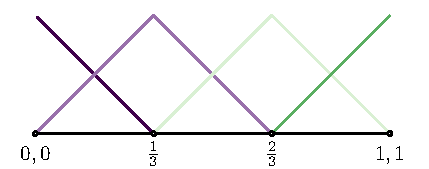
\includegraphics[scale=1.2]{p=1_space}
    \end{subfigure}
    \begin{subfigure}[t]{\linewidth}
        \center
        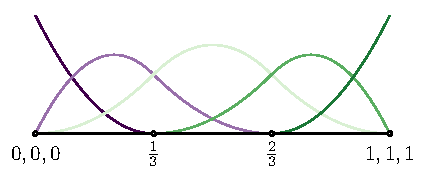
\includegraphics[scale=1.2]{p=2_space}
    \end{subfigure}
    \caption[B-spline basis functions of different degrees.]{B-spline basis functions of different degrees. Top: linear spline basis functions defined by $\left\{0,0,1/3,2/3,1,1\right\}$. Bottom: quadratic spline basis functions defined by $\left\{0,0,0,1/3,2/3,1,1,1\right\}$.}\label{fig:spline_basis}
\end{figure}

B-splines of different degrees are shown in Figure~\ref{fig:spline_basis}. As can be seen, linear B-spline basis functions are identical to the classic hat functions that widely used in finite element analysis. Compared with quadratic Lagrange polynomials in Figure~\ref{fig:lagrange_polynomial}, quadratic B-splines are smoother across each mesh grids. Indeed, B-splines of degree $p$ have up to $p-1$ continuous derivatives. The inter-element continuity can be manipulated by repeating knots. In general, basis functions at knot of multiplicity $m$ are $C^{p-m}$ continuity.

\begin{figure}[ht]
    \center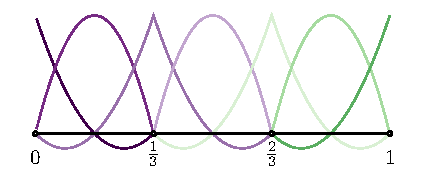
\includegraphics[scale=1.2]{p=2_space_2}
    \caption{Quadratic Lagrange polynomials defined on the same mesh grid as the splines in Figure~\ref{fig:spline_basis}.}\label{fig:lagrange_polynomial}
\end{figure}


A $d$-dimensional B-spline curve $\mathbf{S}(\xi)\in{\R^d}$ can then be defined as
\begin{equation}
    \mathbf{S}(\xi)=\sum_A N_{A,p}(\xi)\mathbf{P}_A
\end{equation}
where $\mathbf{P}_A=(p_A^1,p_A^2,\ldots,p_A^d)^T$ is a $d$-dimensional control point. An example of a B-spline curve is illustrated in Figure~\ref{fig:b-spline_and_geometry}.

\begin{figure}[ht]
    \center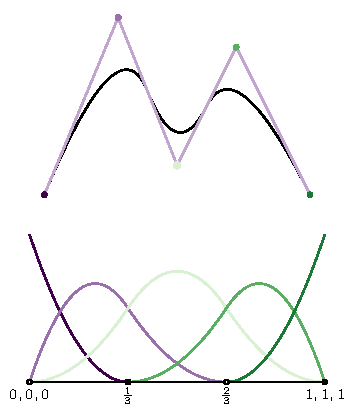
\includegraphics[scale=1.3]{geometry}
    \caption{A B-spline piecewise quadratic curve in $\R^2$ and the corresponding B-spline basis.}\label{fig:b-spline_and_geometry}
\end{figure}

\FloatBarrier
\subsection{The univariate NURBS basis}

B-splines can be used to represent piecewise polynomial functions but are not capable of representing conic sections (e.g. circles, ellipses and hyperbolas). NURBS(Non-Uniform Rational B-Spline) overcome this shortcoming.  A NURBS basis function can be written as
\begin{equation}
    R_{A,p}(\xi)=\dfrac{N_{A,p}(\xi)w_A}{W{(\xi)}}
\end{equation}
where $w_A$ is called a weight and
\begin{align}
    \label{eq:weight}
    W(\xi)=\sum_{A} N_{A,p}(\xi)w_A
\end{align}
is called the weight function. A $d$-dimensional rational curve $\mathbf{S}(\xi)\in{\R^d}$ can then be defined as
\begin{equation}
    \mathbf{S}(\xi)=\sum_A R_{A,p}(\xi)\mathbf{P}_A.
\end{equation}
It is often more convenient to represent the $d$-dimensional NURBS in a $(d+1)$-dimensional homogeneous space by defining $\mathbf{P}_A^w=(p_A^1w_A,p_A^2w_A,\ldots,p_A^dw_A,w_A)^T$ and the corresponding $(d+1)$-dimensional B-spline curve as
\begin{align}
    \mathbf{S}^w(\xi) & =\sum_A N_{A,p}(\xi)\mathbf{P}_A^w
\end{align}
such that each component of $\mathbf{S}^w$ can be written as
\begin{align}
    S_i(\xi) & =\dfrac{{S}_i^w(\xi)}{{S}_{d+1}^w(\xi)}.
\end{align}
In the homogeneous form, NURBS can be manipulated with standard B-spline algorithms.

\subsection{The multivariate spline basis}

In higher dimensions, Bernstein, B-spline, and NURBS basis functions are formed by the Kronecker product of univariate basis functions. For example, two-dimensional B-spline basis functions of degree $\mathbf{p}=(p_\xi, p_\eta)$ are defined by
\begin{equation}
    \mathbf{N}^\mathbf{p}(\xi,\eta)=\mathbf{N}^{p_\xi}(\xi)\otimes\mathbf{N}^{p_\eta}(\eta)
\end{equation}
where $\mathbf{N}^{p_\xi}(\xi)$ and $\mathbf{N}^{p_\eta}(\eta)$ are vectors of basis functions in the $\xi$ and $\eta$ directions, respectively. A particular multivariate basis function can be written as
\begin{equation}
    {N}_{A(i,j)}^\mathbf{p}(\xi,\eta)={N}_{i,p_\xi}(\xi){N}_{j,p_\eta}(\eta)
\end{equation}
where the index mapping is defined as
\begin{equation}
    A(i,j)=n_\eta{i}+j.
\end{equation}
The integer $n_\eta$ is the number of basis functions in $\eta$ direction. In three-dimensional space, a set of basis functions can be constructed by the Kronecker product between two-dimensional basis functions and univariate basis functions.

\section{Geometric Algorithms}\label{sec:geometric_algorithms}

\subsection{Knot insertion}

The knot insertion algorithm ensures the insertion of one or multiple knots into a knot vector $\mathbf{\Xi}$ without changing the shape and parameterization of the curve. It allows us to conduct \textit{h}-refinement (subdividing elements into smaller ones without changing the type of basis functions used) in the context of Isogeometric Analysis. The detailed algorithm of knot insertion can be found in~\cite{piegl2012nurbs}.

An example of knot insertion of the B-spline curve in Figure~\ref{fig:b-spline_and_geometry} is illustrated in Figure~\ref{fig:b-spline_h_refine}. A set of knots $\left\{\frac{1}{6}, \frac{1}{2}, \frac{5}{6}\right\}$ are inserted into the original knot vector $\mathbf{\Xi}=\left\{0,0,0,1/3,2/3,1,1,1\right\}$.  The inserted curve remains geometrically and parametrically identical to the original curve. Meanwhile, knot spans $[ \xi_i,\xi_{i+1} )$ are splitted into smaller ones.

\begin{figure}[ht]
    \center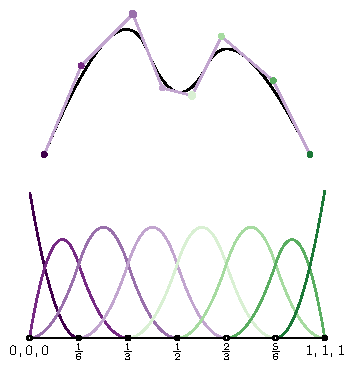
\includegraphics[scale=1.3]{h_refine}
    \caption{Knot insertion for the curve in Figure~\ref{fig:b-spline_and_geometry}. The inserted curve is geometrically and parametrically identical to the original curve.}\label{fig:b-spline_h_refine}
\end{figure}

\subsection{Degree elevation}

The degree elevation algorithm increases the polynomial degree of each B-spline basis functions while preserves the geometry and parameterization of the curve. It allows us to conduct \textit{p}-refinement (increasing the degree of basis functions without changing the number of element used) in the context of Isogemetric Analysis. The detailed algorithm of degree elevation can be found in~\cite{piegl2012nurbs}.

An example of degree elevation of the B-spline curve in Figure~\ref{fig:b-spline_and_geometry} is illustrated in Figure~\ref{fig:b-spline_p_refine}, where the original quadratic spline curve is elevated to cubic and the shape remains unchanged. Recalling that the basis is $C^{p-m}$ continuous at a knot of multiplicity $m$, it is clear that, to preserve the inter-element continuity, the multiplicity of each knots must be increased as the increase of the polynomial degree. In Figure~\ref{fig:b-spline_p_refine}, the multiplicity each knot is increased by one.

\begin{figure}[ht]
    \center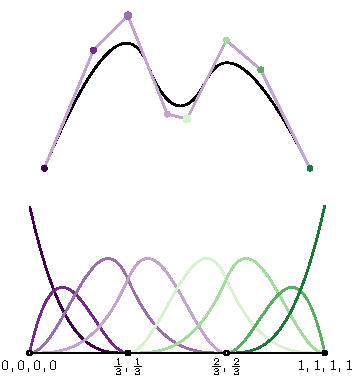
\includegraphics[scale=1.3]{p_refine}
    \caption{Degree elevation for the curve in Figure~\ref{fig:b-spline_and_geometry}. The degree elevated curve is geometrically and parametrically identical to the original curve.}\label{fig:b-spline_p_refine}
\end{figure}

\subsection{\Bezier extration}

\Bezier extraction is a technique that is often used to facilitate the incorporation of isogeometric analysis into existing finite element codes~\cite{borden2011isogeometric,scott2011isogeometric}. \Bezier extraction defines an injection that maps a space spanned by B-spline basis to a space spanned by piecewise Bernstein basis. \Bezier extraction is accomplished by repeating all interior knots of a knot vector until they have a multiplicity equal to $p+1$. The interior knots repeating process defines a linear operator $\mathbf{C}$ (see~\cite{borden2011isogeometric}) such that
\begin{equation}
    \mathbf{N}(\xi)=\mathbf{C}\mathbf{B}(\xi).
\end{equation}
The localization of $\mathbf{C}$ to an element domain produces the element extraction operator $\mathbf{C}^e$.
Given control points $\mathbf{P}^e$, the corresponding B\'ezier control points $\mathbf{Q}^e$ can be computed directly as
\begin{equation}
    \mathbf{Q}^e=(\mathbf{C}^e)^T\mathbf{P}^e.
\end{equation}
A graphical depiction of B\'{e}zier extraction over an element is shown in Figure~\ref{fig:element_extraction_projection}.

\begin{figure}
    \centering
    \begin{subfigure}{\linewidth}
        \center
        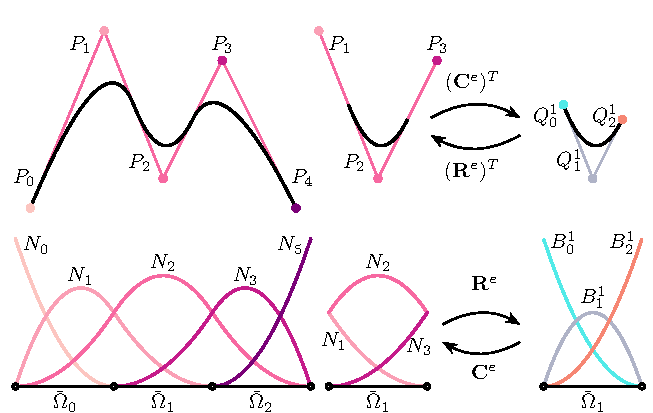
\includegraphics[width=.7\linewidth]{elements_global.pdf}
        \caption{}\label{fig:element_extraction_projection}
    \end{subfigure}
    \begin{subfigure}{\linewidth}
        \center
        \includestandalone[scale = .8]{bezier_extraction_demo}
        \caption{}\label{fig:bezier_extraction_process}
    \end{subfigure}
    \caption{Illustration of \Bezier extraction and projection in one dimension for a B-spline of degree 2 and knot vector $\left\{0,0,0,1/3/2/3,1,1,1\right\}$. (a) The element extraction and projection for the second element. (b) \Bezier extraction over the entire domain.}
\end{figure}

It is possible to view \Bezier projection as a global assembly procedure. The B-spline basis vector $\mathbf{N}$ of dimension $n_N$ can be represented by a set of Bernstein basis functions $\mathbf{B}$ of dimension $n_B$ defined on each element as
\begin{equation}
	\mathbf{N} = \mathbf{A}^T\mathbf{C}\mathbf{B},
\end{equation}
where $\mathbf{C}$ is a block diagonal matrix with \Bezier element extraction operators on the diagonal and the rectangular assembly operator $\mathbf{A}$ is the permutation matrix that maps local element degrees of freedom to global degrees of freedom. The assembly operator $\mathbf{A}$ satisfies the following properties:
\begin{itemize}
	\item Each row of $\mathbf{A}$ contains a single unity-valued entry; all other entries are zero.
	\item Each column of $\mathbf{A}$ contains at most $p+1$ unity-valued entries; all other entries are zero.
	\item Compact support. The non-zero entries can be associated to no more than $p+1$ consecutive elements.
	\item If we consider the column vectors $\mathbf{A}_i$ of $\mathbf{A}$, the space $\spn\left\{\mathbf{A}_i\right\}_{i=0}^{n_N-1}$ is an $n_N$ dimensional subspace of $\mathbb{R}^{n_B}$ and $\left\{\mathbf{A}_i\right\}_{i=0}^{n_N-1}$ are orthogonal, i.e.
	      \begin{equation}
		      \mathbf{A}_i\cdot\mathbf{A}_j\neq{}0\iff{i=j}.
	      \end{equation}
\end{itemize}

The \Bezier extraction process for the quadratic B-spline basis defined by the knot vector $\{0,0,0,1/3,2/3,1,1,1\}$ is shown in Fig.~\ref{fig:bezier_extraction_process}. The assembly operator $\mathbf{A}$ for this example is given by
\begin{equation}\label{eq:assembly_matrix}
	\mathbf{A} =
	\begin{blockarray}{cccccc}
		N_0 & N_1  & N_2  & N_3  & N_4 \\
		\begin{block}{[ccccc]c}
			1 & \hfsetfillcolor{hred!10}\hfsetbordercolor{hred}\tikzmarkin{a}(0.1,-0.1)(-0.1,0.35)0 & 0 & 0 & 0 & N_0^0 \\
			0 & 1 & 0 & 0 & 0 & N_1^0 \\
			0 & 0 & 1 & 0 & 0 & N_2^0 \\
			0 & 1 & 0 & 0 & 0 & N_0^1 \\
			0 & 0 & 1 & 0 & 0 & N_1^1 \\
			0 & 0 & 0\tikzmarkend{a} & 1 & 0 & N_2^1 \\
			0 & 0 & 1 & 0 & 0 & N_0^2 \\
			0 & 0 & 0 & 1 & 0 & N_1^2 \\
			0 & 0 & 0 & 0 & 1 & N_2^2 \\
		\end{block}
	\end{blockarray},
\end{equation}
where the highlighted submatrix is the restriction of $\mathbf{A}$ onto elements $\Omega_0$ and $\Omega_1$, and onto the B-spline basis functions $N_1$ and $N_2$.

\subsection{B\'ezier projection}
\label{sec:bproject}

B\'{e}zier projection can be viewed as the inverse of extraction~\cite{thomas_bezier_2015}. It defines an surjection that maps a space spanned by  piecewise Bernstein basis onto a space spanned by B-spline basis. B\'ezier projection uses an element reconstruction operator $\mathbf{R}^e\equiv(\mathbf{C}^e)^{-1}$ such that the global control point values, corresponding to those basis functions defined over the support of an element $e$, can be determined directly from \Bezier control values as
\begin{equation}
    \mathbf{P}^e=(\mathbf{R}^e)^T\mathbf{Q}^e
\end{equation}
where $\mathbf{Q}^e$ is any field in B\'ezier form. The action of the element reconstruction operator is depicted graphically in Figure~\ref{fig:element_extraction_projection}. For example, given any function $u \in L^2$, we can compute $\mathbf{Q}^e$ as
\begin{equation}
    \mathbf{Q}^e=(\mathbf{G}^e)^{-1}\mathbf{F}^e
    \label{eq:element-Qi}
\end{equation}
where $\mathbf{G}^e$ is the Gramian matrix corresponding to the Bernstein basis with components
\begin{align}
    {G}_{ij}^e & = \int_{\Omega^e} B^e_i B^e_j \, d\Omega =\langle{B^e_{i},B^e_{j}}\rangle_{\Omega^e}\label{eq:element_gramian}
\end{align}
and
\begin{align}
    {F}^e_i & =  \int_{\Omega^e} B^e_i u \, d\Omega = \langle{B^e_{i,},u}\rangle_{\Omega^e}.
\end{align}
Note that efficiency gains can be had at the expense of accuracy by instead performing the integration in the parametric domain of the element~\cite{thomas_bezier_2015}.

The element-wise projection produces one control value for each element in the support of the function.  These values must be combined in order to provide the final control value.  A core component of the B\'ezier projection algorithm is the definition of an appropriate averaging operation. The process of computing the weights is illustrated in Figure~\ref{fig:weights}. A weighted average of the values is computed using the weighting
\begin{equation}\label{eq:Bezier_weight}
    \omega_a^e=\dfrac{\int_{\Omega^e} N_{a}^e \, d\Omega}{\int_{\Omega^A} N_{A(e,a)} \, d\Omega}
\end{equation}
where $\Omega^e$ corresponds to the physical domain of element $e$, $A(e,a)$ is a mapping from a local nodal index $a$ defined over element $e$ to a corresponding global node index $A$, and $\Omega^A$ corresponds to the physical support of $N_A$. The final averaged global control point is then calculated as
\begin{equation}
    P_A=\sum_{\Omega^e\in \Omega^A } \omega_{A(e,a)} P_{A(e,a)}.
\end{equation}
B\'ezier projection onto NURBS functions can be defined in an analogous manner~\cite{thomas_bezier_2015}.

The individual steps comprising the \Bezier projection algorithm are
illustrated in Figure~\ref{fig:loc-proj-example} where
the curve defined by $\vec{f}(t)=\left( \frac{t}{3}
    \right)^{3/2}\vec{e}_1+\frac{1}{10}\sin (\pi t )\,\vec{e}_2$,
$t\in[0,3]$ is projected onto the quadratic B-spline basis defined by
the knot vector $\left\{0,0,0,\frac{1}{3},\frac{2}{3},1,1,1\right\}$. For this example,
the algorithm proceeds as follows:

\begin{description}

    \item{Step 1:} The function $\mathbf{f}$ is projected onto the Bernstein basis of each element. This results in a set of
          \Bezier coefficients that define an approximation to $\mathbf{f}$.
          The \Bezier coefficients are indicated in part (1) of Figure~\ref{fig:loc-proj-example} by
          square markers that have been colored to match the corresponding
          element. Each \Bezier segment is discontinuous.

    \item{Step 2:} The element reconstruction operator $\mathbf{R}^e$ is used to convert the
          \Bezier control points into spline control points associated with the
          basis function segments over each element.
          The new control points are marked with inverted triangles and
          again colored to indicate the element with which the control point is
          associated. The control points occur in clusters.
          The clusters of control points represent the contributions from
          multiple elements to a single spline basis function control point.

    \item{Step 3:} Each cluster of control points is averaged to obtain a
          single control point by weighting each point in the cluster according
          to the weighting given in (\ref{eq:Bezier_weight}). The resulting control
          points are shown as circles with the relative contribution from each
          element to each control point indicated by the colored fraction of the
          control point marker. Colors in Figures~\ref{fig:weights} and~\ref{fig:loc-proj-example} are coordinated
          to illustrate where the averaging weights come from and their values.
\end{description}

\begin{figure}[htb]
    \centering
    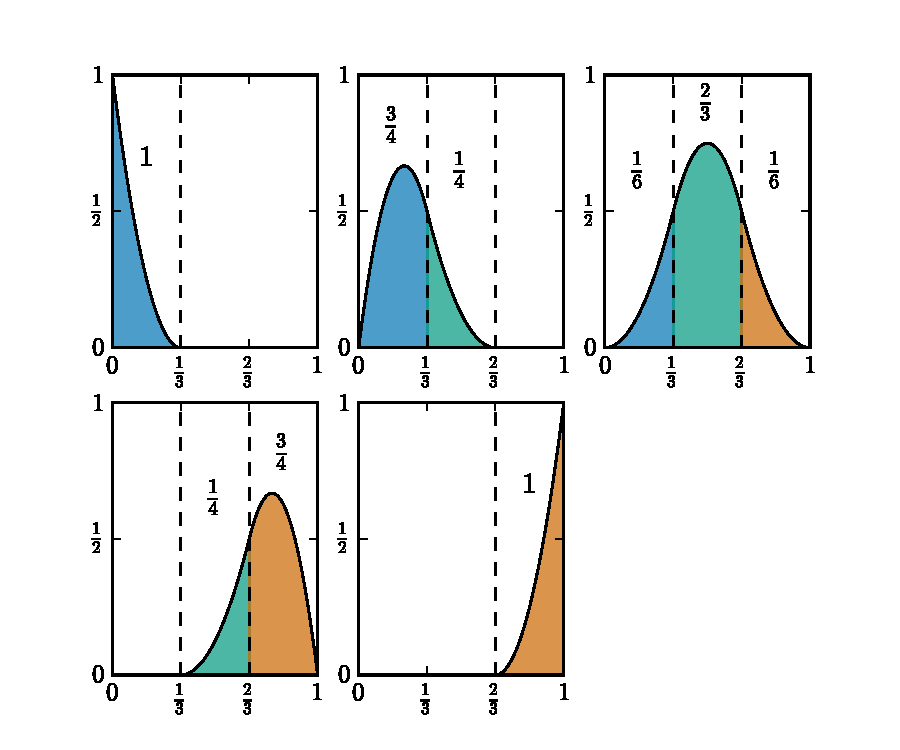
\includegraphics[width=5in]{weights.pdf}
    \caption{\label{fig:weights}Weights over each knot span associated
        with the basis function defined by the knot vector
        $[0,0,0,\frac{1}{3},\frac{2}{3},1,1,1]$.}
\end{figure}
\begin{figure}[htb]
    \centering
    \begin{tabular}{c p{4in} p{2in}}
        (0) & \raisebox{-.5\height}{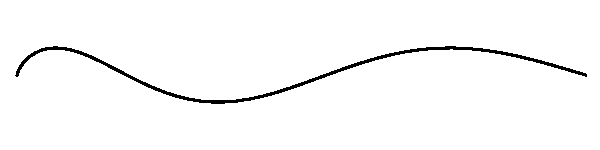
\includegraphics[width=4in]{local_proj_steps1.pdf}} & \begin{minipage}[t]{2in}Target function\end{minipage} \\
        (1) & \raisebox{-.5\height}{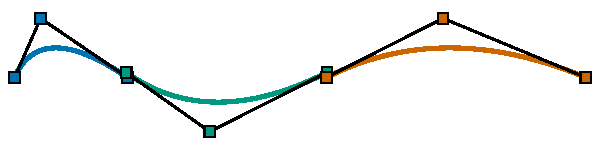
\includegraphics[width=4in]{local_proj_steps2.pdf}} & \begin{minipage}[t]{2in}Perform local projection to obtain \Bezier control points (represented by squares, colored to match elements)\end{minipage} \\
        (2) & \raisebox{-.5\height}{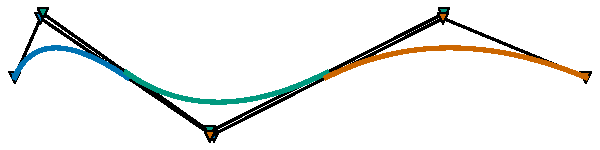
\includegraphics[width=4in]{local_proj_steps3.pdf}} & \begin{minipage}[t]{2in}Use element reconstruction operator to project \Bezier points to spline control points (represented by inverted triangles, colored to match elements)\end{minipage} \\
        (3) & \raisebox{-.5\height}{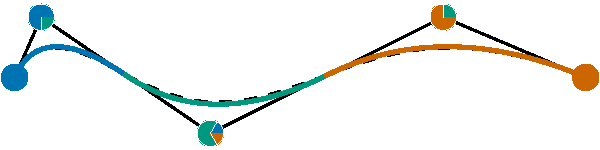
\includegraphics[width=4in]{local_proj_steps4.pdf}} & \begin{minipage}[t]{2in}Apply smoothing algorithm (contribution of each element to each control point shown by colored fraction)\end{minipage} \\
        (4) & \raisebox{-.5\height}{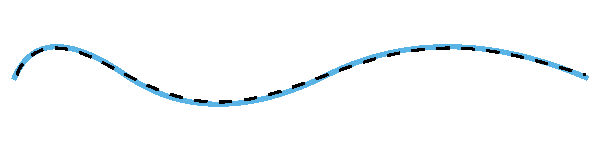
\includegraphics[width=4in]{local_proj_steps5.pdf}} & \begin{minipage}[t]{2in}Comparison of final function (light blue) and target function (dashed)\end{minipage}
    \end{tabular}
    \caption{\label{fig:loc-proj-example}Steps of \Bezier projection.}
\end{figure}

\section{Dual basis}\label{sec:dual_basis}
%%TODO: bezier dual basis function will be used for what?
In this section, we give a brief introduction to the concept of global and \Bezier dual basis functions. \Bezier dual basis functions will be used in Section to facilitate the solution of domain coupling problems in the dual mortar method. A dual basis is defined as a set of basis functions $\{\hat{N}_i\}_{i=1}^{n}$, which are dual to a corresponding set of primal basis functions $\{{N}_i\}_{i=1}^{n}$ in the sense that
\begin{equation}\label{eq:def:dual}
    \langle\hat{N}_i,N_j\rangle_\Omega:=\int_\Omega\hat{N}_iN_jd\Omega=\delta_{ij}, \quad\forall{}i,j\in\left[1,2,\dots,n\right],
\end{equation}
where $\delta_{ij}$ is the Kronecker delta.

\subsection{Global dual basis}

The global dual basis functions  $\{\hat{N}_i^G\}_{i=1}^{n}$ for a given set of primal basis function $\{{N}_i\}_{i=1}^{n}$ can be computed as
\begin{equation}
    \hat{N}_i^G=\sum_j G^{-1}_{ij}N_j,\label{eq:global_dual}
\end{equation}
where  $G^{-1}_{ij}$ are the components of the inverse of the Gramian matrix $\mathbf{G}$ with components $G_{ij}=\langle{N}_i,N_j\rangle_\Omega$.


In Isogeometric Analysis, we choose B-spline functions as the primal basis. One important property of B-spline functions is that they have compact support. This leads to sparse linear systems when these functions are used to define the trial and weighting function spaces in a Galerkin method. The global dual basis functions, however, do not have compact support and will result in dense linear systems when used as the weighting function space in a Galerkin method. Dual basis supports are shown in Figure~\ref{fig:bezier_extraction_illustration} where we have highlighted one B-spline function in Figure~\ref{fig:b-spline-func} and then shown the corresponding global dual basis function in Figure~\ref{fig:global_dual}.

\begin{figure}[ht]
    \center
    \begin{subfigure}{\linewidth}
        \center
        \includestandalone[scale=1]{basisfunctions}
        \caption{}\label{fig:b-spline-func}
    \end{subfigure}
    \begin{subfigure}{\linewidth}
        \center
        \includestandalone[scale=1]{dual_global_one}
        \caption{}\label{fig:global_dual}
    \end{subfigure}
    \begin{subfigure}{\linewidth}
        \center
        \includestandalone[scale=1]{bezier_dual_one}
        \caption{}\label{fig:bezier_dual}
    \end{subfigure}
    % or use \input{mytikz}
    \caption{A comparison of a B-spline basis function (a) with the corresponding global dual basis function (b) and the \Bezier dual basis function (c).}
    \label{fig:bezier_extraction_illustration}
\end{figure}

\subsection{\Bezier dual basis}

To maintain the sparsity of linear systems we will use \Bezier dual basis functions, which are computed locally and have compact support. These functions are computed using the \Bezier projection operator introduced in~\cite{thomas_bezier_2015}. The \Bezier dual basis has been shown to be effective in reducing volumetric and shear locking~\cite{MIAO2018273}, alleviating membrane locking in Kirchhoff-Love shells~\cite{greco2018reconstructed}, and as a dual mortaring strategy for elasticity problems~\cite{zou2018isogeometric}.

The construction of \Bezier dual basis functions leverages \Bezier extraction/projection~\cite{borden2011isogeometric, thomas2015bezier} and can be performed in several simple steps. For a given \Bezier element, $\Omega_e$, the element extraction operator $\mathbf{C}^e$ is computed. The element extraction operator maps a set of Bernstein polynomials $\{B_i\}_{i=1}^m$ defined over a \Bezier element, where $m$ depends on the polynomial degree of the \Bezier element in each parametric direction, into the set of global B-spline basis functions that have support over that element. The element reconstruction operator, $\mathbf{R}^e$, and the Gramian matrix, $\mathbf{G}^{e}$~\eqref{eq:element_gramian}, of the Bernstein polynomials defined over the element are then computed. The element extraction operator for the dual basis is then simply
\begin{equation}
    \hat{\mathbf{D}}^e=\text{diag}(\omega^e)\mathbf{R}^e\left[\mathbf{G}^{e}\right]^{-1}
\end{equation}
where $\text{diag}(\omega^e)$ is a diagonal matrix with the \Bezier projection weights~\eqref{eq:Bezier_weight} on the diagonal.

The restriction of a \Bezier dual basis functions $\hat{N}_i^B$ to $\Omega_e$ is then computed as
\begin{equation}
    \hat{N}^B_i\vert_{\Omega_e}=\sum_{j=1}^m\hat{D}^e_{ij}B_j.\label{eq:bezier-dual-basis}
\end{equation}
From this local definition of the dual basis over an element we have
\begin{equation}
    \int_{\Omega_e}\hat{N}^B_iN_jd\Omega=\omega^e_i\delta_{ij},
\end{equation}
and
\begin{equation}
    \A_e{} \int_{\Omega_e}\hat{N}^B_iN_jd\Omega=\delta_{ij},
\end{equation}
where $\A$ is the standard assembly operator \cite{Hug00} . The \Bezier dual basis of the B-spline basis function highlighted in Figure~\ref{fig:b-spline-func} is shown in Figure~\ref{fig:bezier_dual}. Note that the \Bezier dual basis function has the same compact support as the primal B-spline basis function.

\subsection{Rational dual basis functions}
If rational basis functions are used, the construction of the dual basis must be modified slightly. A rational dual basis must satisfy the biorthogonality requirement
\begin{align}
    \int_{\Omega} \bar{R}_A R_B \, d\Omega= \delta_{AB}.
\end{align}
A simple way to achieve biorthogonality is to define
\begin{align}
    \bar{R}_A & = W \bar{N}_A/w_A
\end{align}
where $W$ is the rational weight given in (\ref{eq:weight}). Now
\begin{align}
    \int_{\Omega} \bar{R}_A R_B \, d\Omega & = \int_{\Omega} \bar{N}_A N_B \, d\Omega = \delta_{AB}.
\end{align}

\begin{remark}
    The \Bezier dual basis functions define a quasi-interpolation operator $\mathcal{T}(f)=\sum_i \langle\hat{N}^B_i,f\rangle N_i$, which possesses the following properties:
    \begin{itemize}
        \item Optimal approximation: for $p^\text{th}$ order spline basis function and $f\in C^\infty$, the approximation error is given by~\cite{thomas_bezier_2015}
              \begin{equation}
                  \|\mathcal{T}(f)-f\|_{L^2}\leq Ch^{p+1}\|f\|_{H^{p+1}}.
              \end{equation}
        \item Boundary interpolation: for two sets of $p^\text{th}$ order spline basis functions $\{{N^s_i}\}_{i=1}^{n_s}$ and $\{{N^m_i}\}_{i=1}^{n_m}$ defined on $\left[{0,L}\right]$, if the first and last elements of $s$ are subsets of the first and last elements of $m$, then
              \begin{equation}
                  \mathcal{T}^s(f^m)(0)=f^m(0)\;\text{ and }\;\mathcal{T}^s(f^m)(L)=f^m(L),\quad\forall f^m\in\spn\{{N^m_i}\}_{i=1}^{n_m}.\label{eq:boundary_interpolation}
              \end{equation}
    \end{itemize}
    The second property is critical for the coercivity of the biharmonic problem on multi-patch domains.
\end{remark}

%%%%%%%%%%%%% begin Bibliography %%%%%%%%%%%%%%%%%
\cleardoublepage
\bibliographystyle{IEEEtran}
\bibliography{exampleFiles/refs} % Use your own BibTex file here

% Include appendix sections here: (or comment these lines out to have no appendices)
\appendix
\chapter{Making a Figure with Width Based on Page Size}
\label{apdx:appendixa}

\section{Width Based on Page Size Figure Example} \label{sec:appendixa_figure_example}
Here's an example of a figure whose width depends on the width
of the page. You can see it as Figure~\ref{fig:appendix_some_pic}. This also shows another citation \cite{aeyels86local}.

\begin{figure}[htbp]
  \centering
  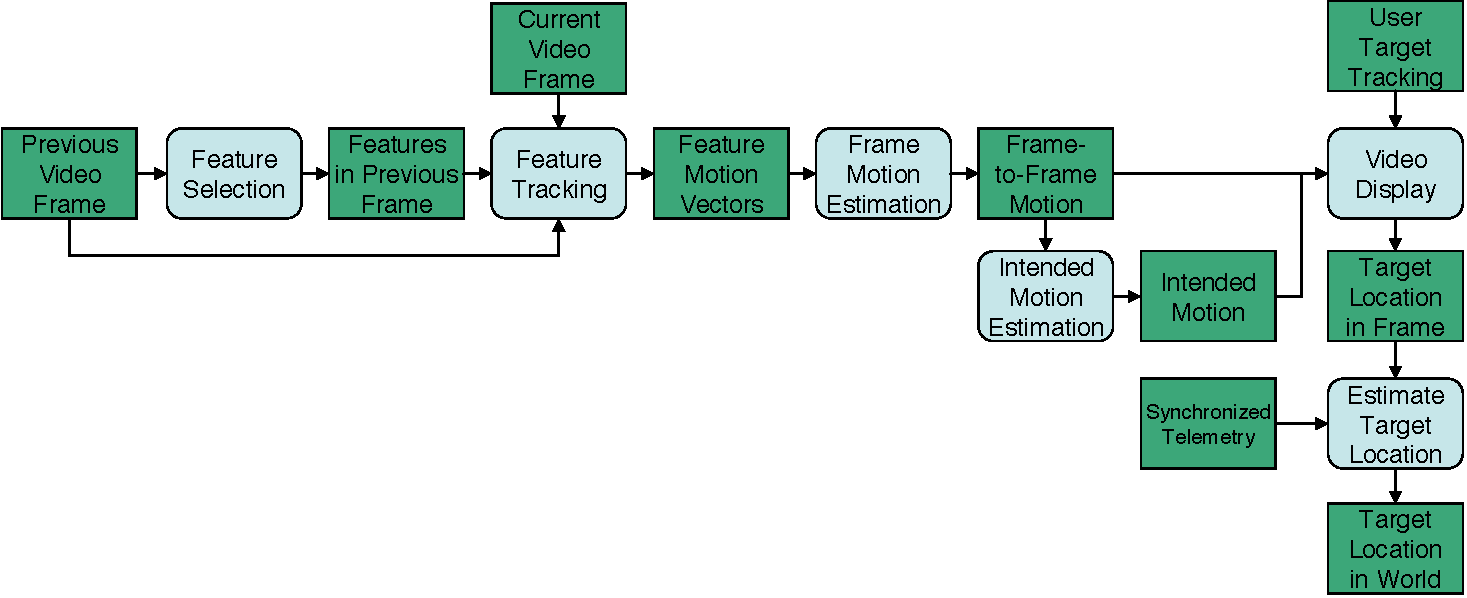
\includegraphics[width=0.45\textwidth]{exampleFiles/some_pic}
  \caption[Example figure whose width depends on page size]{
    This is an example of a figure whose width will be 45\% of the
    width of the page. If you'd like to see a figure with a fixed
    width then you can see it as Figure~\ref{fig:intro_stuff} in
    Section~\ref{sec:intro_figure_example} of Chapter~\ref{chp:chapter1}.}
  \label{fig:appendix_some_pic}
\end{figure}
\chapter{Formatting Guidelines for Thesis}
\label{apdx:appendixb}

This appendix outlines the required formatting for theses and dissertations. While the \LaTeX\ template takes care of most of these automatically, it is the student's responsibility to ensure that all formatting requirements are incorporated in the document.

\section{Font} Times New Roman 12 pt. throughout text and 10 or 11 point for tables and figures.

\section{Margins}
\begin{itemize}
\item Preliminary Pages (Title page, Abstract page(s), Acknowledgment page, Table of Contents, List of Figures, List of Tables):
1 inch on all sides
\item Body Pages, beginning with Introduction:
1 inch on all sides
\item Chapter title pages, Appendix title page, Reference title page:
2 inches at top,
1 inch at bottom and sides
\end{itemize}

\section{Printing}
\begin{itemize}
\item Single-sided: Title page, Abstract page(s), Acknowledgment page
\item Two-sided:  Table of Contents, List of Figures, List of Tables, Body, Appendix, References
\end{itemize}
Note:  Table of Contents, List of Figures, List of Tables, Chapter title pages, References and Appendix pages must begin on the front side of a page.

\section{Page Numbering}
\begin{itemize}
\item	Page numbers are centered at the bottom of the page.
\item	Counting begins with the Title page; however, back pages are not counted until the Table of Contents.
\item	Page numbers do not appear on the page until the Table of Contents (v).
\item	Use Roman Numerals (v, vi, vii, ...) for the Table of Contents page and the pages thereafter until Chapter 1.  
\item	Use Arabic numbers (1, 2, 3 ...) beginning with Chapter 1. 
\item	Be sure numbers appear on all blank back pages once numbering begins.
\end{itemize}

\section{Spacing}
\begin{itemize}
\item	Double-space text of body.
\item	Single-space abstract, captions, quotes, long chapter titles, headings, and subheadings.
\item	Table of Contents, List of Figures, List of Tables, and References can be single-spaced or double spaced.
\item	Double-space three times after chapter titles (48 pts).
\item	Double-space twice before subheadings (24 pts). 
\item	Double-space once after subheadings (0 pts). 
\item	Double-space once between two subheadings (0 pts). 
\item	Double-space twice before and after figures (24 pts).
\item	Double-space twice before and after tables (24 pts).
\item	Double-space once before and after equations (0 pts).
\item	Do not leave a single line of text, a single-line equation, or a subheading alone on the top (widow) or bottom (orphan) of a page.
\item	Do not leave more than about 5 lines of white space remaining on a page unless it's the end of a chapter.
\end{itemize}

\section{Figures}
\begin{itemize}
\item	Figures are normally diagrams, graphs, maps, or charts.
\item	Center figures on the page.
\item	Center captions below the figure. If two lines are needed, the caption should be left justified at margin.
\item	A figure should be placed after the paragraph of reference.  If it will not fit on the same page, continue the text and place the figure on the next page.
\end{itemize}

\section{Tables}
\begin{itemize}
\item	Tables contain numerical or statistical information.
\item	Center tables on the page.
\item	Center captions above the table.  If more than one line is needed, center the lines in an inverted pyramid:                                                          
\begin{singlespace}
\begin{center}Table 6.3 Comparison of roll rotation plots when node was displaced,\\
 and an X-direction off-axis force was applied.\end{center}
\end{singlespace}
\item	If placed in the landscape position, the top of the table should be on the left side of the page, with the caption above the table.  The page number is placed in the standard location.
\end{itemize}

\end{document}